\section{Results} \label{sec:results}

\subsection{Data analysis algorithm}

Data analysis was performed in the following steps:
\begin{enumerate}
\item calculate log returns of the input data to make time series stationary,
\item decompose log returns in Daubechies (\emph{db4} in PyWavelet implementation) wavelet basis,
\item reconstruct data in the original domain for each time scale,
\item test for linear Granger causality using an autoregressive model test for each wavelet scale, for up to 5 steps,
\item test for nonlinear Granger causality using the Diks-Panchenko test for each wavelet scale, for up to 5 steps.
\end{enumerate}

Then, 999 surrogate data sets were generated and the same analysis procedure was perfomed for each realization.
The number of statistically significant results among surrogates divided by number of realizations was used to asses results fidelity.

Statistical significance was assumed for $p$-values less than $0.1$ for both linear and nonlinear tests.

Given 552 monthly observations (45 years) in the analyzed data sets, the wavelet scales correspond to the time scales as presented in \fref{tab:scales} 

\begin{table}[h]
\begin{center}
\begin{tabular}{c|c}
\hline\hline
Wavelet scale & Time scale \\
\hline
D1 & 2-4 months \\
D2 & 4-8 months \\
D3 & 8-16 months \\
D4 & 16-32 months \\
D5 & 32-64 months \\
D6 & 64-128 months \\
A6 & $>$128 months \\
\hline\hline
\end{tabular}
\end{center}
\caption{Wavelet time scales}
\label{tab:scales}
\end{table}

\subsection{Wavelet decomposed data}
Logarithmic returns of the time series are presented in \ref{fig:usd-logret} and \ref{fig:oil-logret}.
Wavelet decomposition of the original data is presented here in figures: \ref{fig:usd-wr-a6}-\ref{fig:oil-wr-d6}.
To depict how different wavelet scales relate to the input data, the logarithmic returns are displayed in light grey in the background of each plot.
An example surrogate data wavelet decomposition is presented in \fref{appendix:wavelet-surrogate}.

\begin{figure}[h]
\begin{center}
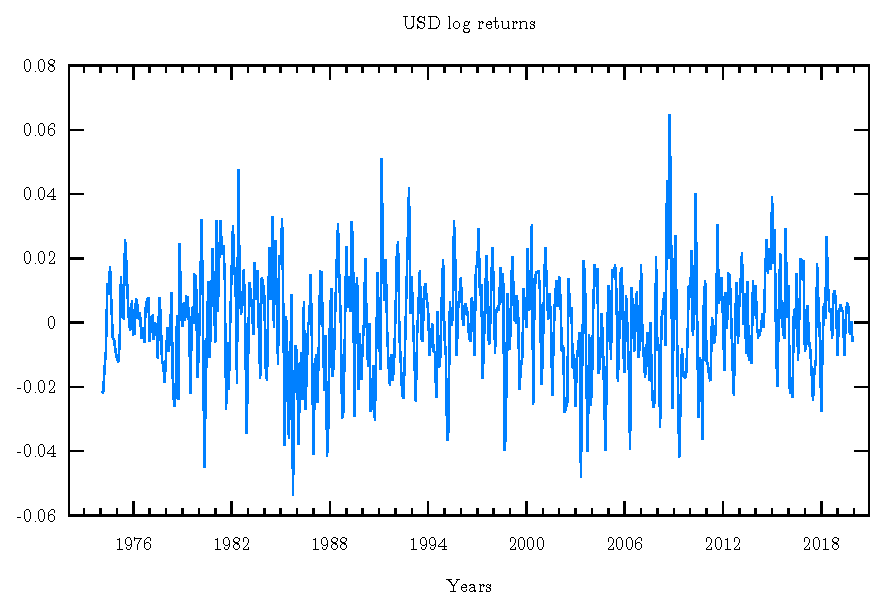
\includegraphics[width=0.8\textwidth]{./code/plot/dollar_logret.eps}
\caption{Plot of log returns of U.S. Dollar Index.}
\label{fig:usd-logret}
\end{center}
\end{figure}

\begin{figure}
\begin{center}
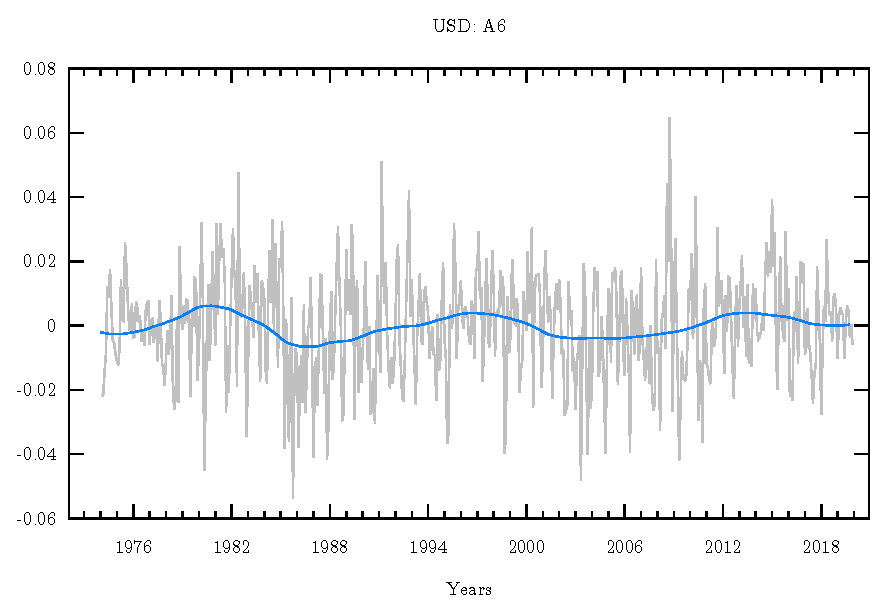
\includegraphics[width=0.8\textwidth]{./code/plot/usd_wr_A6.eps}
\caption{Plot of A6 component of wavelet decomposition of U.S. Dollar Index log returns. 
	Plot of the original data in grey. A6 scale corresponds to $>$128 months.}
\label{fig:usd-wr-a6}
\end{center}
\end{figure}

\begin{figure}
\begin{center}
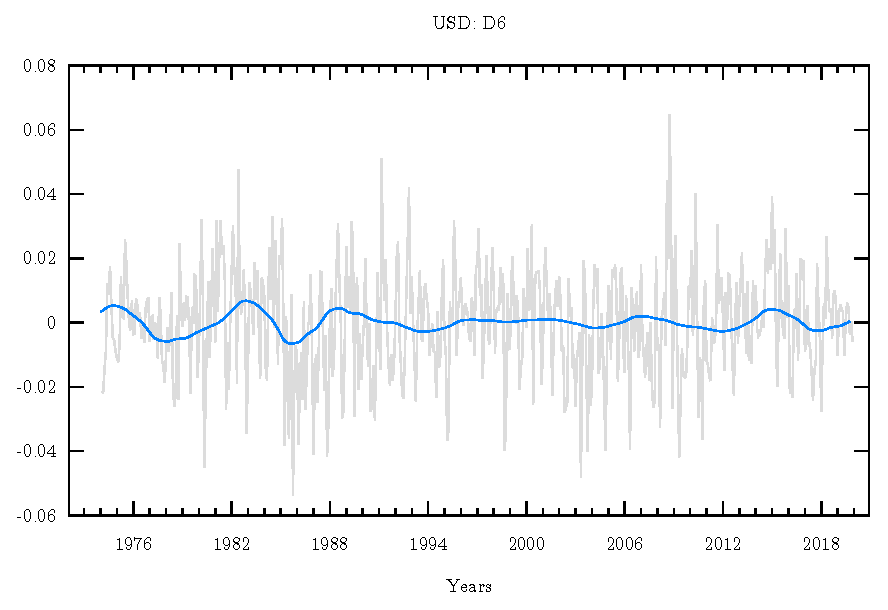
\includegraphics[width=0.8\textwidth]{./code/plot/usd_wr_D6.eps}
\caption{Plot of D6 component of wavelet decomposition of U.S. Dollar Index log returns. 
	Plot of the original data in grey. D6 scale corresponds to 64-128 months.}
\label{fig:usd-wr-d6}
\end{center}
\end{figure}

\begin{figure}
\begin{center}
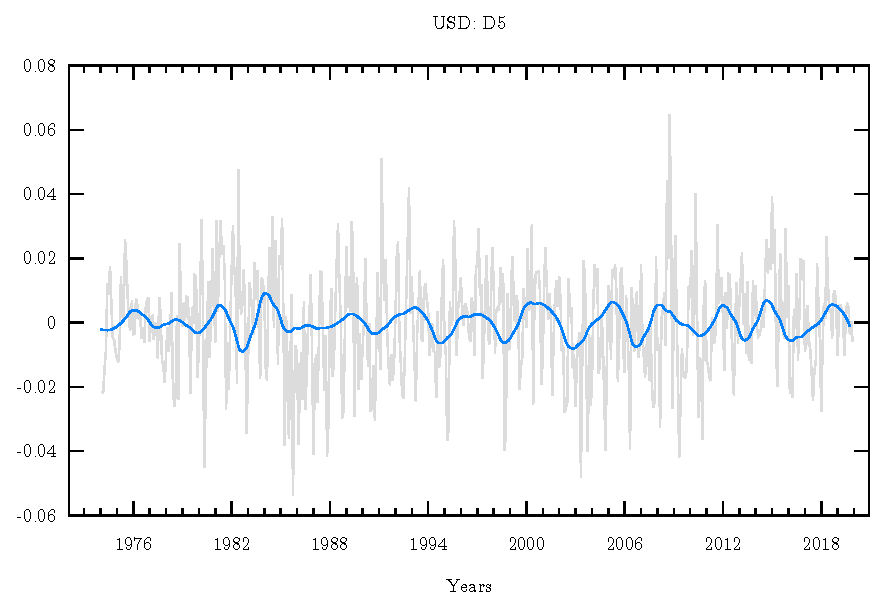
\includegraphics[width=0.8\textwidth]{./code/plot/usd_wr_D5.eps}
\caption{Plot of D5 component of wavelet decomposition of U.S. Dollar Index log returns. 
	Plot of the original data in grey. D5 scale corresponds to 32-64 months.}
\label{fig:usd-wr-d5}
\end{center}
\end{figure}

\begin{figure}
\begin{center}
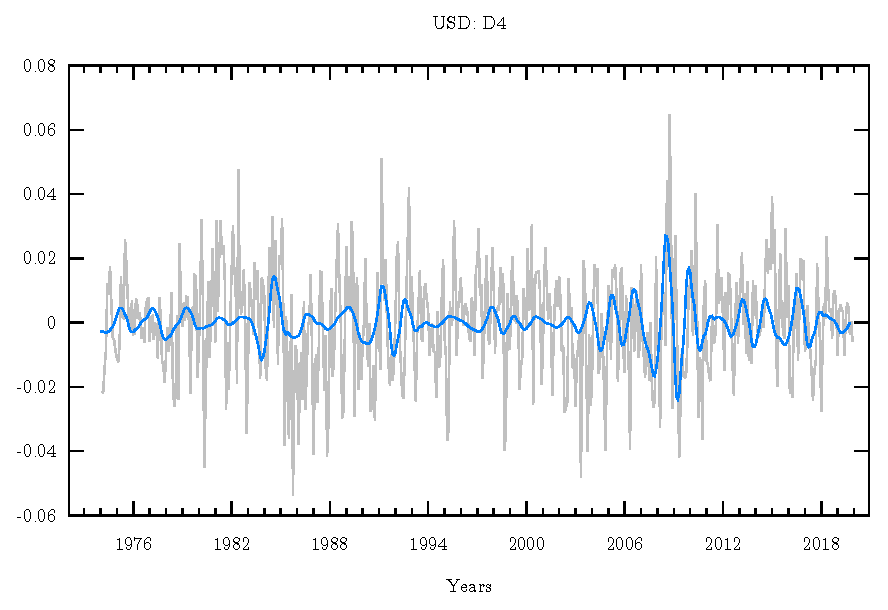
\includegraphics[width=0.8\textwidth]{./code/plot/usd_wr_D4.eps}
\caption{Plot of D4 component of wavelet decomposition of U.S. Dollar Index log returns. 
	Plot of the original data in grey. D4 scale corresponds to 16-32 months.}
\label{fig:usd-wr-d4}
\end{center}
\end{figure}

\begin{figure}
\begin{center}
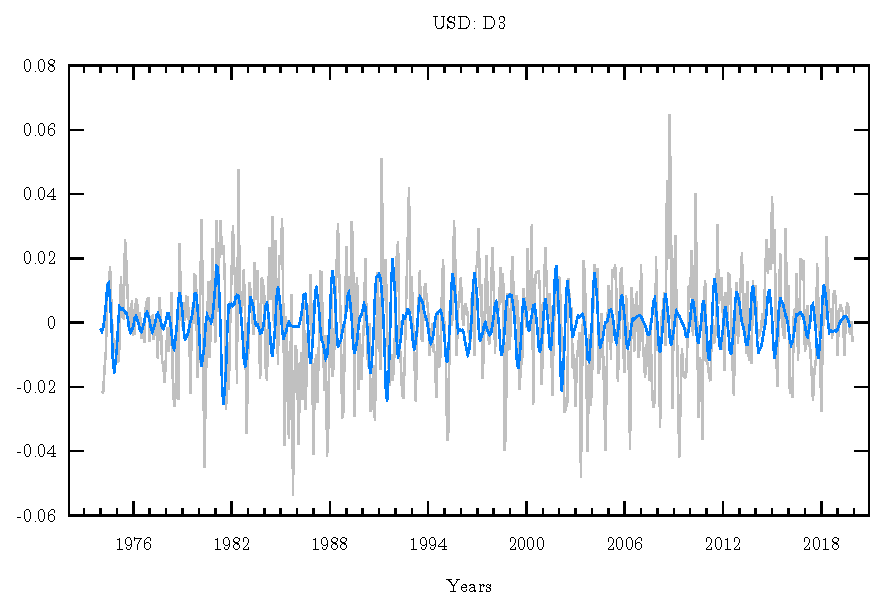
\includegraphics[width=0.8\textwidth]{./code/plot/usd_wr_D3.eps}
\caption{Plot of D3 component of wavelet decomposition of U.S. Dollar Index log returns. 
	Plot of the original data in grey. D3 scale corresponds to 8-16 months.}
\label{fig:usd-wr-d3}
\end{center}
\end{figure}

\begin{figure}
\begin{center}
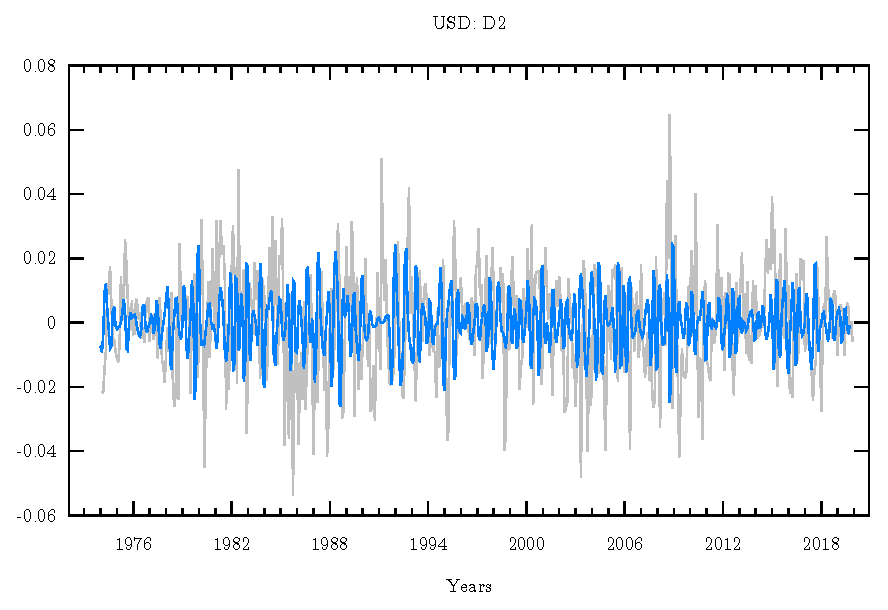
\includegraphics[width=0.8\textwidth]{./code/plot/usd_wr_D2.eps}
\caption{Plot of D2 component of wavelet decomposition of U.S. Dollar Index log returns. 
	Plot of the original data in grey. D2 scale corresponds to 4-8 months.}
\label{fig:usd-wr-d2}
\end{center}
\end{figure}

\begin{figure}
\begin{center}
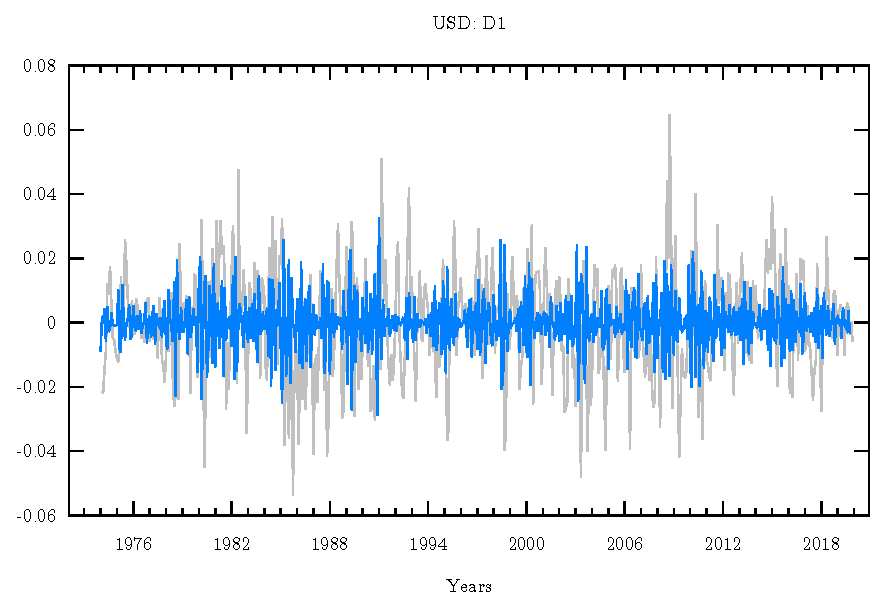
\includegraphics[width=0.8\textwidth]{./code/plot/usd_wr_D1.eps}
\caption{Plot of D1 component of wavelet decomposition of U.S. Dollar Index log returns. 
	Plot of the original data in grey. D1 scale corresponds to 2-4 months.}
\label{fig:usd-wr-d1}
\end{center}
\end{figure}

\begin{figure}
\begin{center}
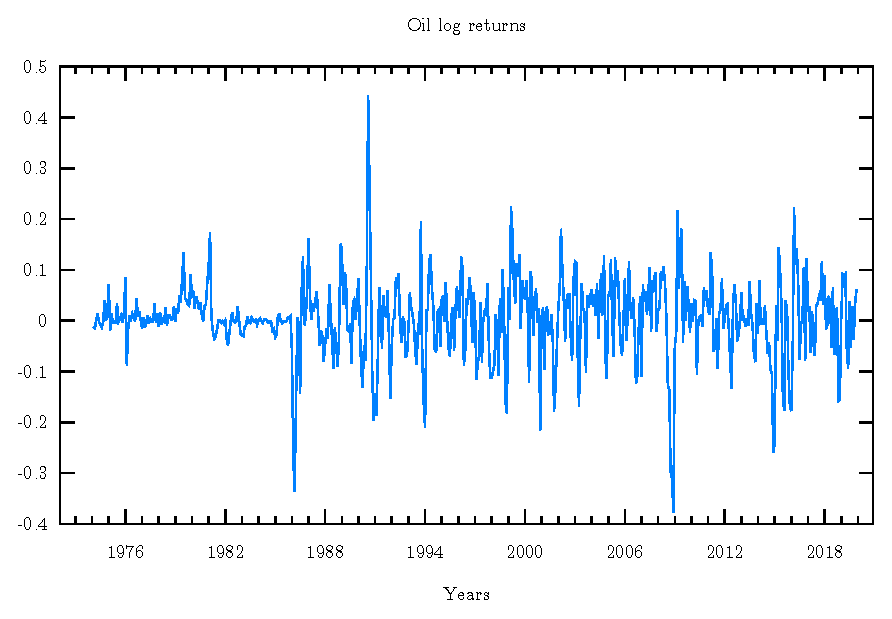
\includegraphics[width=0.8\textwidth]{./code/plot/oil_logret.eps}
\caption{Plot of log returns of oil price.}
\label{fig:oil-logret}
\end{center}
\end{figure}

\begin{figure}
\begin{center}
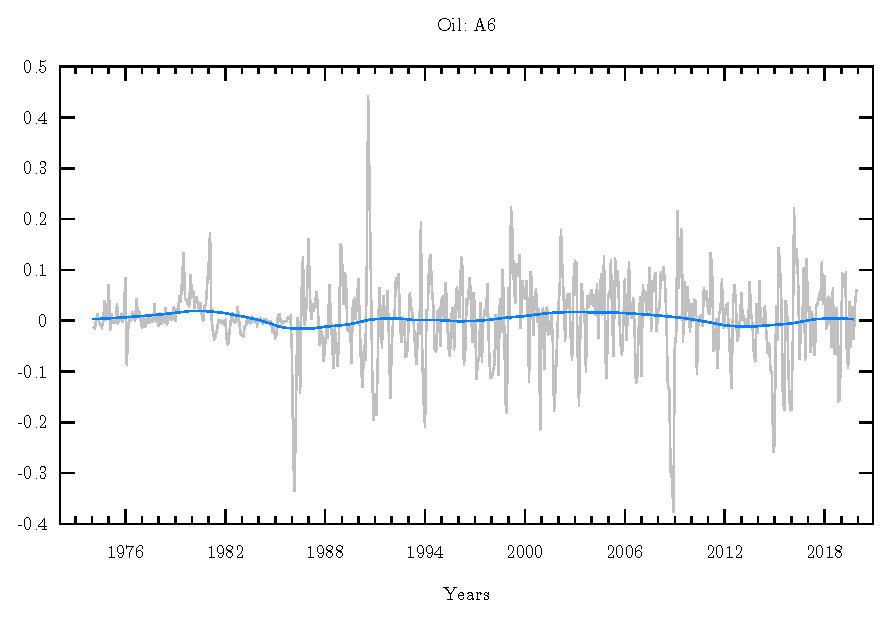
\includegraphics[width=0.8\textwidth]{./code/plot/oil_wr_A6.eps}
\caption{Plot of A6 component of wavelet decomposition oil price  log returns. 
	Plot of the original data in grey. A6 scale corresponds to $>$128 months.}
\label{fig:oil-wr-a6}
\end{center}
\end{figure}

\begin{figure}
\begin{center}
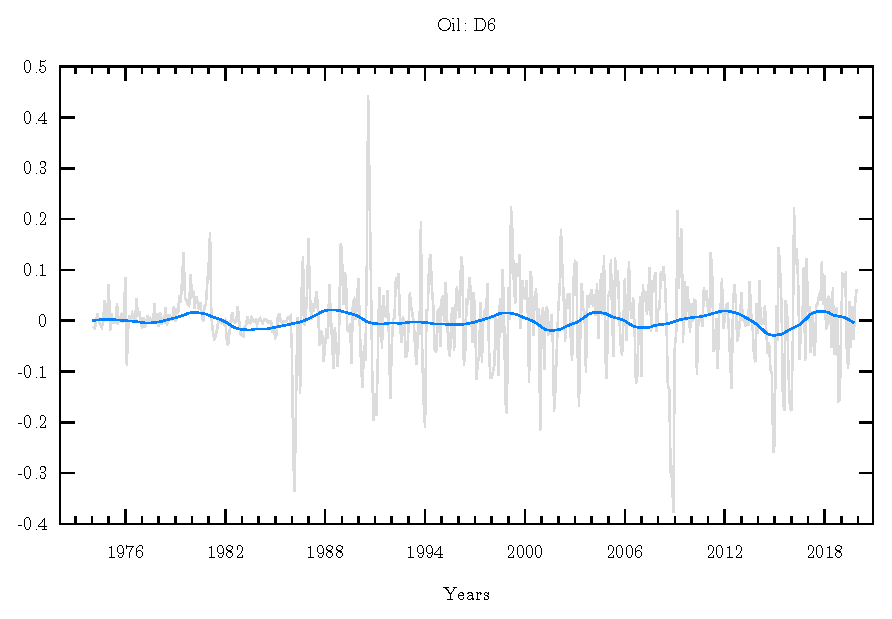
\includegraphics[width=0.8\textwidth]{./code/plot/oil_wr_D6.eps}
\caption{Plot of D6 component of wavelet decomposition of oil price log returns. 
	Plot of the original data in grey. D6 scale corresponds to 64-128 months.}
\label{fig:oil-wr-d6}
\end{center}
\end{figure}

\begin{figure}
\begin{center}
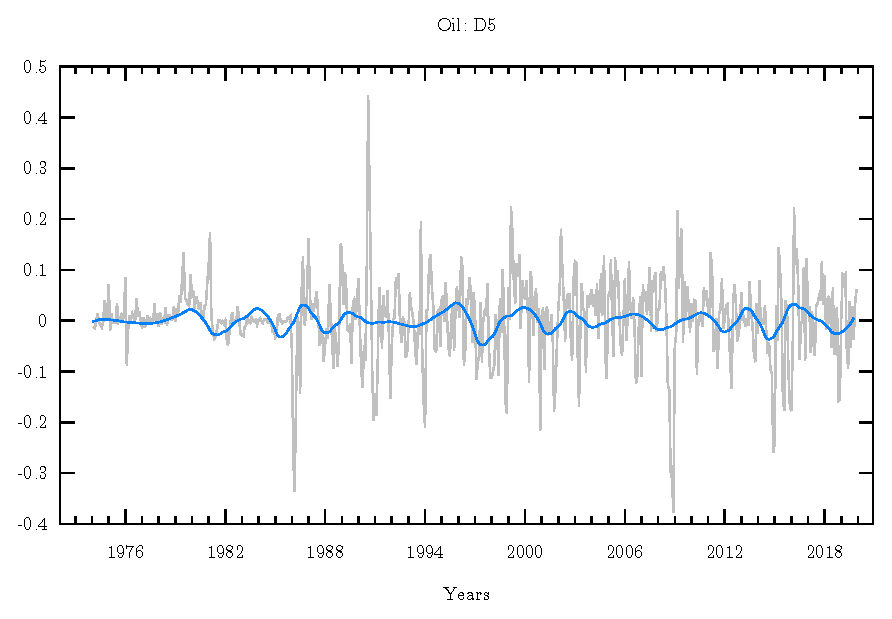
\includegraphics[width=0.8\textwidth]{./code/plot/oil_wr_D5.eps}
\caption{Plot of D5 component of wavelet decomposition of oil price log returns. 
	Plot of the original data in grey. D5 scale corresponds to 32-64 months.}
\label{fig:oil-wr-d5}
\end{center}
\end{figure}

\begin{figure}
\begin{center}
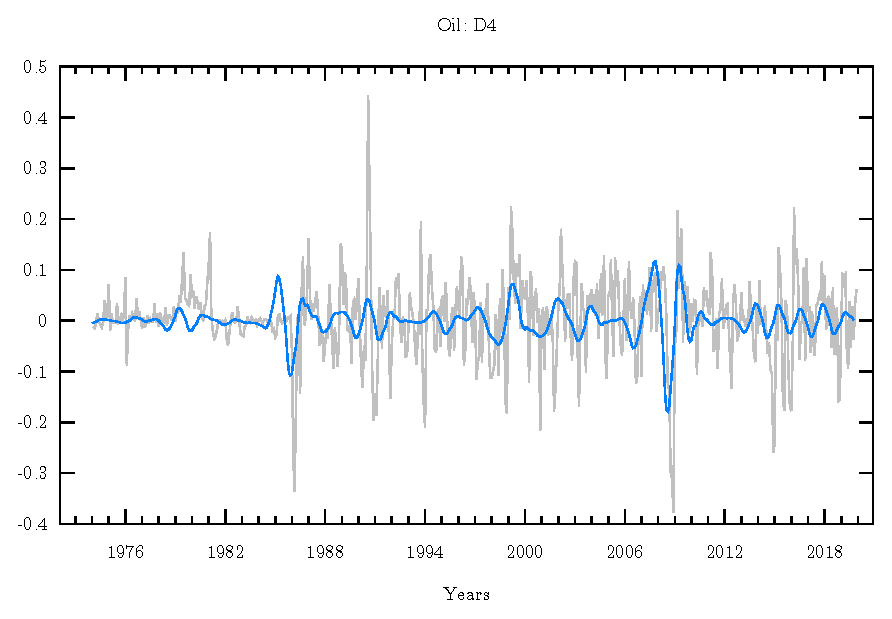
\includegraphics[width=0.8\textwidth]{./code/plot/oil_wr_D4.eps}
\caption{Plot of D4 component of wavelet decomposition of oil price log returns. 
	Plot of the original data in grey. D4 scale corresponds to 16-32 months.}
\label{fig:oil_wr_d4}
\end{center}
\end{figure}

\begin{figure}
\begin{center}
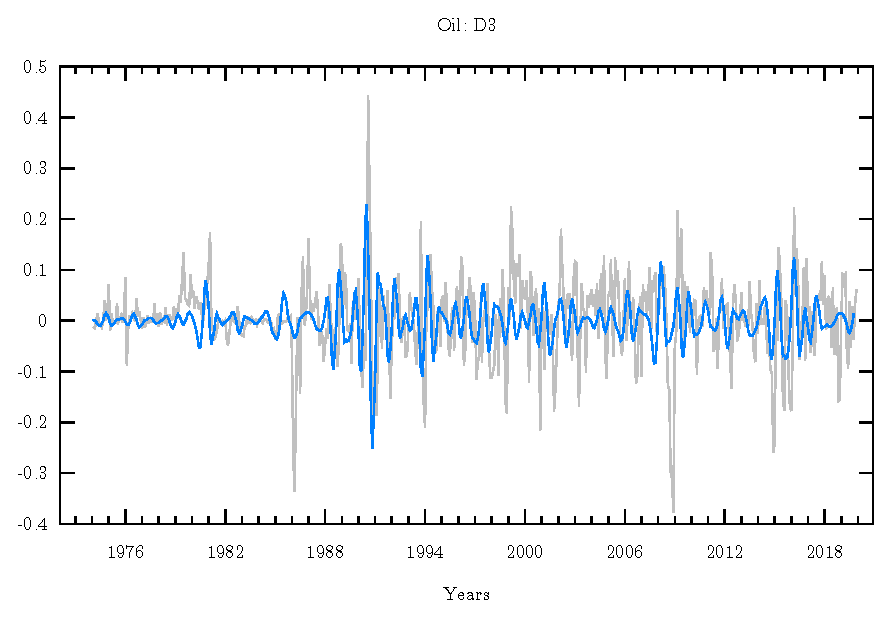
\includegraphics[width=0.8\textwidth]{./code/plot/oil_wr_D3.eps}
\caption{Plot of D3 component of wavelet decomposition of oil price log returns. 
	Plot of the original data in grey. D3 scale corresponds to 8-16 months.}
\label{fig:oil-wr-d3}
\end{center}
\end{figure}

\begin{figure}
\begin{center}
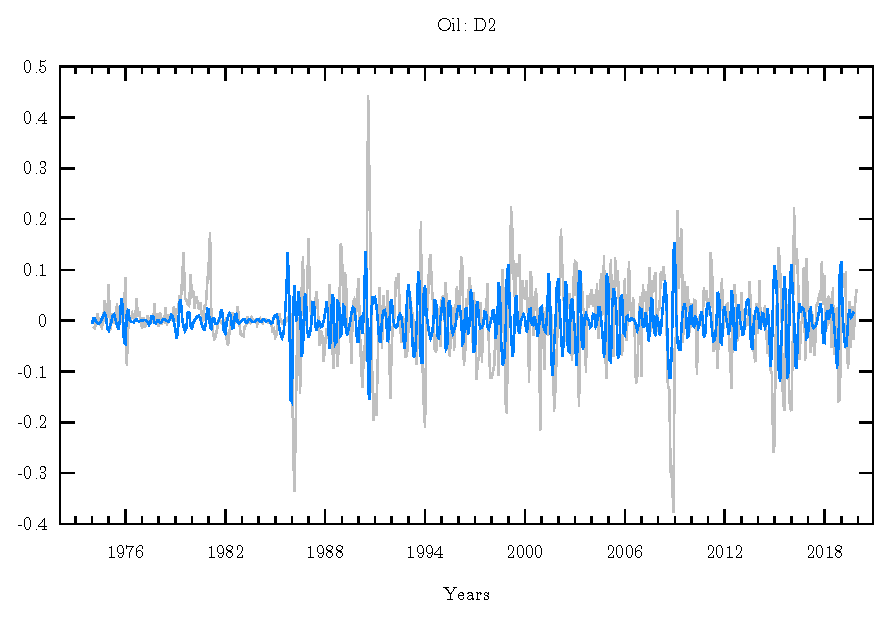
\includegraphics[width=0.8\textwidth]{./code/plot/oil_wr_D2.eps}
\caption{Plot of D2 component of wavelet decomposition of oil price log returns. 
	Plot of the original data in grey. D2 scale corresponds to 4-8 months.}
\label{fig:oil-wr-d2}
\end{center}
\end{figure}

\begin{figure}
\begin{center}
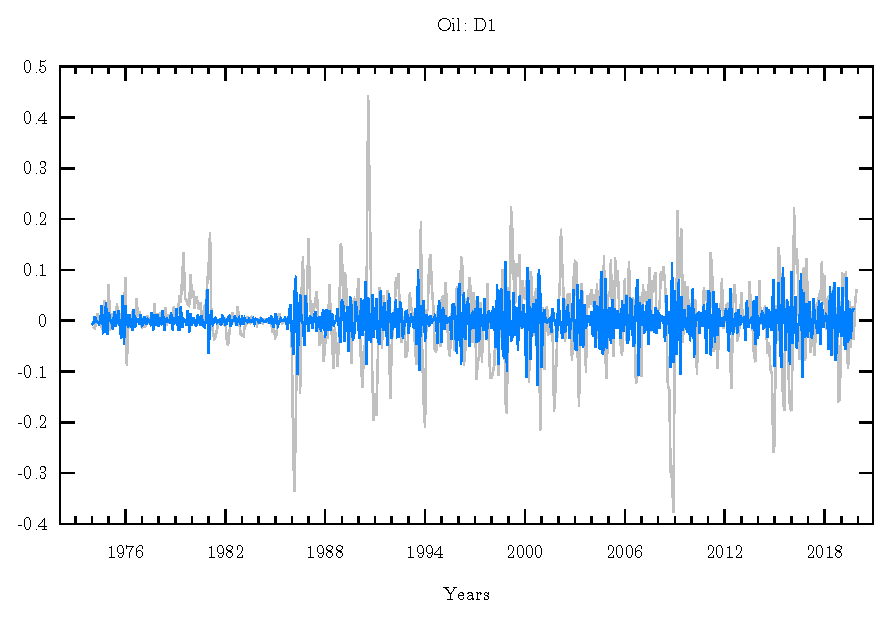
\includegraphics[width=0.8\textwidth]{./code/plot/oil_wr_D1.eps}
\caption{Plot of D1 component of wavelet decomposition of oil price log returns. 
	Plot of the original data in grey. D1 scale corresponds to 2-4 months.}
\label{fig:oil-wr-d1}
\end{center}
\end{figure}

\newpage
\subsection{Causality tests results}

\subsubsection{Linear causality test results}
Linear causality is or is not. There is no inbetween.

\begin{table}[h]
\begin{center}
\begin{tabular}{l|r r r r r r r}
\multicolumn{8}{c}{USD $\Rightarrow$ Oil}\\
\hline\hline
m & A6 & D6 & D5 & D4 & D3 & D2 & D1 \\
\hline
1 & 0.5582 & \cellcolor{mygreen}0.0000 & \cellcolor{mygreen}0.0000 & 0.8945 & \cellcolor{mygreen!50}0.0863 & \cellcolor{mygreen!50}0.0824 & 0.6077 \\
2 & 0.3072 & 0.3164 & 0.3697 & 0.1483 & \cellcolor{mygreen!50}0.0712 & 0.5719 & 0.9694 \\
3 & 0.7976 & 0.6942 & 0.6056 & 0.4365 & 0.1070 & 0.2071 & 0.8897 \\
4 & 0.8522 & 0.6486 & 0.7137 & 0.2195 & 0.1190 & 0.2170 & 0.8114 \\
5 & 0.8267 & 0.6394 & 0.4607 & 0.5841 & \cellcolor{mygreen}0.0416 & 0.4541 & 0.8830 \\
6 & 0.8109 & 0.7697 & 0.2951 & 0.3344 & 0.2618 & 0.9708 & 0.9700 \\
\hline\hline
\end{tabular}
\caption{p-values for linear Granger causality test under $H_0$:\\
\mbox{U.S. Dollar Index} does not cause oil price. Statistical significance assumed for $p<0.1$.}
\end{center}
\end{table}

\subsubsection{Nonlinear causality test results}
Sometimes there is, sometimes there isn't.

\begin{table}
\begin{center}
\begin{tabular}{l|r r r r r r r}
\multicolumn{8}{c}{Oil $\Rightarrow$ USD}\\
\hline\hline
m & A6 & D6 & D5 & D4 & D3 & D2 & D1 \\
\hline
1 & 0.7546 & \cellcolor{mygreen}0.0000 & \cellcolor{mygreen}0.0001 & 0.4996 & \cellcolor{mygreen}0.0041 & \cellcolor{mygreen}0.0263 & 0.6923 \\
2 & 0.4907 & \cellcolor{mygreen!50}0.0959 & 0.3098 & 0.4793 & \cellcolor{mygreen}0.0121 & 0.2096 & 0.9649 \\
3 & 0.9205 & 0.3837 & 0.5776 & 0.7582 & \cellcolor{mygreen}0.0048 & \cellcolor{mygreen}0.0104 & 0.9484 \\
4 & 0.9368 & 0.2978 & 0.7321 & 0.6207 & \cellcolor{mygreen}0.0009 & \cellcolor{mygreen}0.0078 & 0.9617 \\
5 & 0.9647 & 0.3165 & 0.5454 & 0.8233 & \cellcolor{mygreen}0.0000 & \cellcolor{mygreen}0.0315 & 0.9889 \\
6 & 0.9647 & 0.3674 & 0.3357 & 0.7435 & \cellcolor{mygreen}0.0000 & 0.1749 & 0.9987 \\
\hline\hline
\end{tabular}
\caption{p-values for linear Granger causality test under $H_0$:\\
oil price does not cause U.S. Dollar Index. Statistical significance assumed for $p<0.1$.}
\end{center}
\end{table}

\subsection{Surrogate data results}
Inconclusive.

\section{Conclusions} \label{sec:conclusions}

